\chapter{Giới thiệu}
\label{chap:gioithieu}

\section{Động cơ của đề tài}
\label{sec:dongco}

\subsection{Bối cảnh và thực trạng}
\label{sec:thuctrang}

Chuỗi cung ứng nông sản truyền thống tại Việt Nam vẫn phụ thuộc nặng vào các khâu trung gian: nông sản thường đi qua 4--5 khâu trước khi đến tay người tiêu dùng, khiến giá thành bị đội lên 30--40\% so với giá tại trang trại \parencite{tapchicongthuong_ipsard_2023_2024}, trong khi phần lớn nông dân vẫn giao dịch qua kênh tự do do thương lái định giá (Hình~\ref{fig:thuctrang}). Thương lái vừa giải quyết bài toán thu gom, sơ chế, vận chuyển mà nông hộ nhỏ khó tự làm, vừa có vị thế ép giá do nắm thông tin thị trường tốt hơn và thường là điểm bán duy nhất tại địa phương vào vụ thu hoạch rộ \parencite{vilas_logistics} (bất cân xứng thông tin --- mục~\ref{subsec:reputation}).

\begin{figure}[t]
\centering
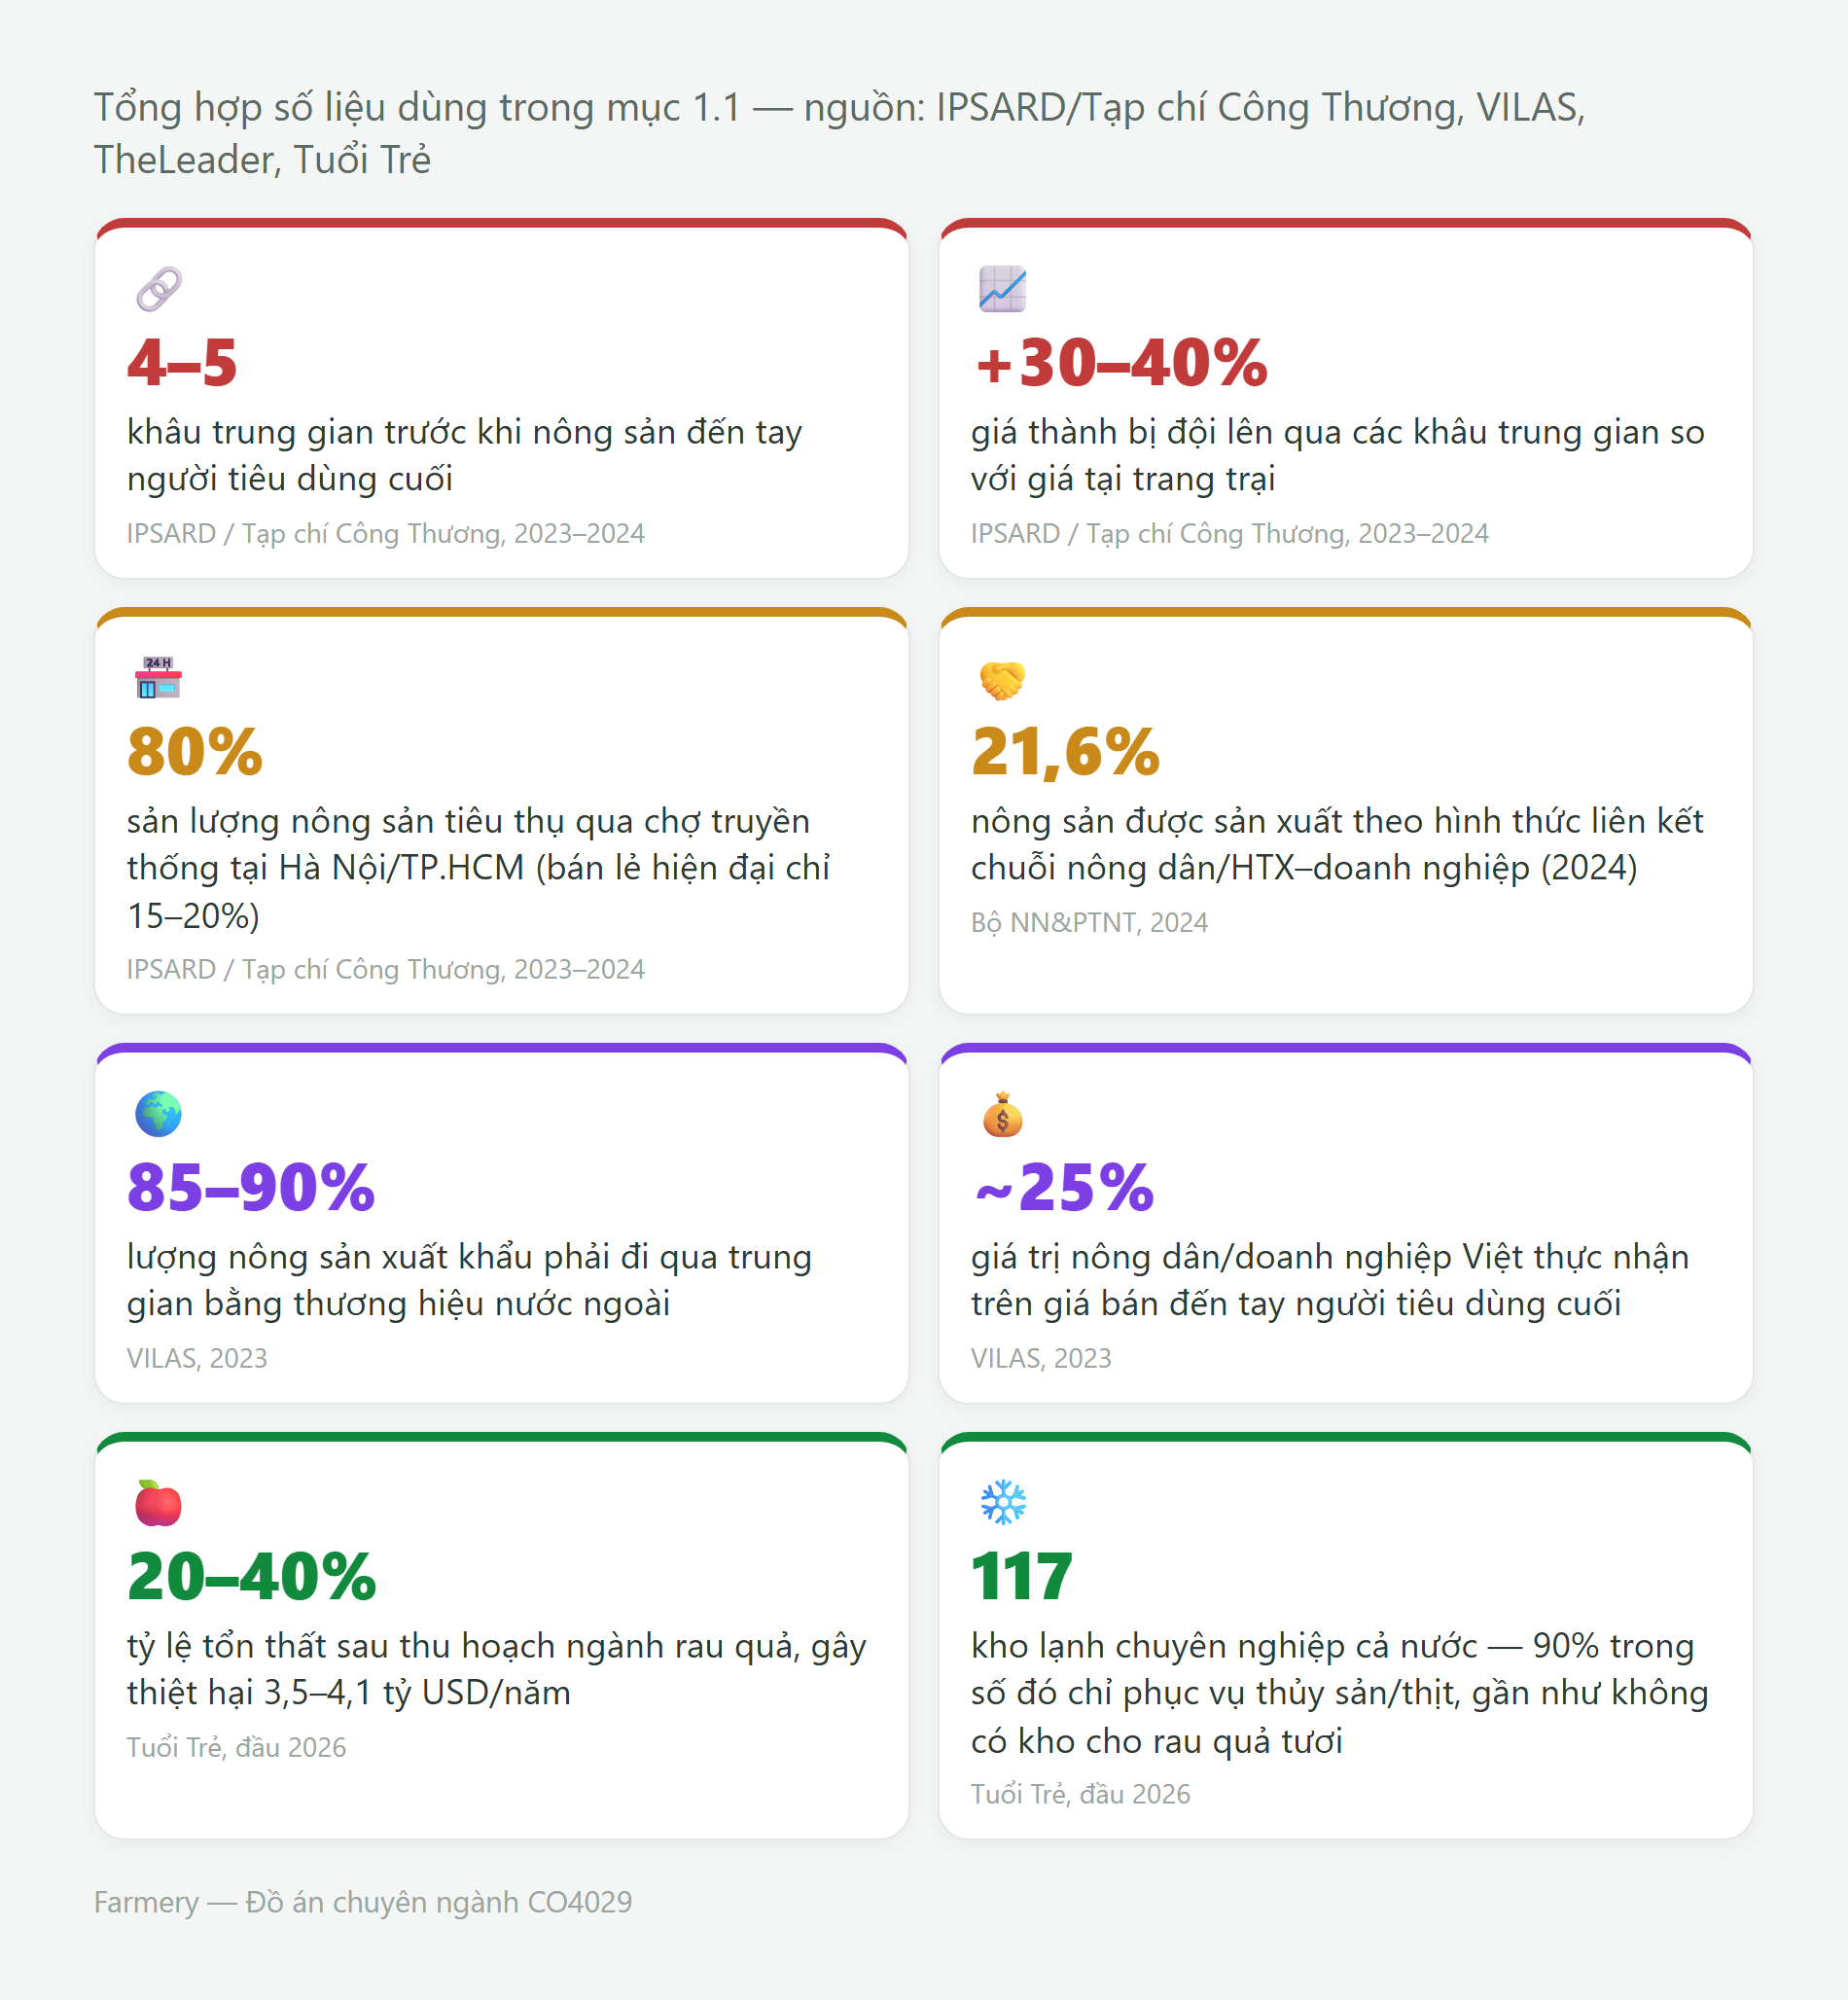
\includegraphics[width=0.85\textwidth]{image/comparison/thuc-trang-chuoi-cung-ung.png}
\caption{Thực trạng chuỗi cung ứng nông sản Việt Nam}
\label{fig:thuctrang}
\end{figure}

Thực trạng này gắn với bản chất mặt hàng: nông sản tươi mau hỏng, sản lượng dồn theo mùa vụ, chất lượng không đồng nhất giữa các lô và người mua không tự kiểm chứng được chất lượng. Vì vậy nông sản không được phục vụ tốt bởi các nền tảng thương mại điện tử thiết kế cho hàng công nghiệp (phân tích tại mục~\ref{sec:dacdiemnongsan}).

\subsection{Vấn đề cần giải quyết}
\label{sec:vande}

Đồ án xác định bốn vấn đề dẫn tới hiện tượng ``được mùa mất giá'' và sự thiếu tin cậy trên thị trường nông sản:

\begin{enumerate}
    \item[\textbf{V1.}] \textbf{Cung dồn theo mùa vụ:} sản lượng tăng ồ ạt khi vào vụ do sản xuất theo tập quán, thiếu thông tin nhu cầu để quy hoạch rải vụ.
    \item[\textbf{V2.}] \textbf{Thiếu kênh tiêu thụ:} nông dân thiếu phương án tiêu thụ đa kênh và năng lực bảo quản, chế biến để hấp thụ sản lượng dư, nên vẫn phụ thuộc thương lái địa phương.
    \item[\textbf{V3.}] \textbf{Hao hụt sau thu hoạch và thiếu kho lạnh:} tỷ lệ hao hụt một số loại trái cây có thể lên tới 35--40\% \parencite{theleader_2024}; toàn ngành rau quả tổn thất 20--40\%, tương ứng thiệt hại 3,5--4,1 tỷ USD mỗi năm, và tình trạng thiếu kho lạnh chưa cải thiện đáng kể tới đầu năm 2026 \parencite{tuoitre_2026}. Nông dân buộc phải ``bán ngay, bán vội'', càng yếu thế khi đàm phán giá.
    \item[\textbf{V4.}] \textbf{Thiếu minh bạch nguồn gốc và niềm tin:} người mua khó phân biệt nông sản ``sạch'' thật với sản phẩm chỉ gắn mác marketing; theo lý thuyết bất cân xứng thông tin (mục~\ref{subsec:reputation}), người bán hàng chất lượng cao không chứng minh được giá trị thực nên mất động lực sản xuất theo tiêu chuẩn.
\end{enumerate}

\section{Mục tiêu}
\label{sec:muctieu}

\subsection{Mục tiêu tổng quát và mục tiêu cụ thể}

Xây dựng Farmery --- nền tảng thương mại điện tử chuyên biệt cho nông sản, vận hành đồng thời hai luồng: sàn bán sỉ nơi nông dân và hợp tác xã tự bán cho doanh nghiệp, và gian hàng bán lẻ nơi chính nền tảng thu mua rồi bán lại cho người tiêu dùng --- nhằm góp phần giải quyết bốn vấn đề tại mục~\ref{sec:vande}. Cụ thể:

\begin{enumerate}
    \item[\textbf{MT1.}] Quy trình đăng ký, xác thực và kiểm duyệt chứng nhận cho nhà cung cấp.
    \item[\textbf{MT2.}] Truy xuất nguồn gốc bằng mã QR gắn với nhật ký canh tác theo từng lô.
    \item[\textbf{MT3.}] Luồng bán sỉ tối giản: yêu cầu báo giá, hợp đồng có xác nhận giao kết, giá bậc theo MOQ, giao một đợt; thiết kế đầy đủ phần giao nhiều đợt và ký quỹ.
    \item[\textbf{MT4.}] Luồng bán lẻ theo mô hình tự thu mua và bán lại: đơn thu mua, nghiệm thu, tồn kho theo lô, đóng gói kèm tem QR, định giá bán.
    \item[\textbf{MT5.}] Trục bán lẻ phía khách hàng: giỏ hàng, thanh toán, theo dõi đơn, giao hàng ba chặng, đổi trả và hoàn tiền, phù hợp hàng dễ hư hỏng.
    \item[\textbf{MT6.}] Tính năng AI hỗ trợ ra quyết định: tìm kiếm theo ngữ nghĩa, gợi ý sản phẩm tương tự; mô hình dự báo giá phục vụ thu mua (chạy offline).
    \item[\textbf{MT7.}] Công cụ quản trị gồm kiểm duyệt và giám sát vi phạm; thiết kế phần báo cáo thống kê.
\end{enumerate}

\subsection{Mục tiêu đánh giá hệ thống}
\label{sec:muctieudanhgia}

Kết quả được kiểm chứng bằng số đo thay vì mô tả định tính, theo bốn nhóm định hướng Chương~\ref{chap:danhgia}: (i) \textbf{chức năng} --- bộ test case phủ các nhóm yêu cầu và luồng nghiệp vụ chính; (ii) \textbf{hiệu năng và độ tin cậy} --- thời gian phản hồi, chịu tải, toàn vẹn dữ liệu, trọng tâm là chống bán vượt tồn kho khi một lô được giao dịch song song ở hai luồng; (iii) \textbf{mô-đun AI} --- chỉ số phù hợp từng bài toán, đối chiếu ngưỡng đặt trước khi hiện thực; (iv) \textbf{khả dụng} --- thử với đại diện các nhóm người dùng, trong đó nông dân và hợp tác xã là phép thử khó nhất. Hạng mục không đánh giá được bằng số trong điều kiện đồ án thì chuyển sang hướng phát triển (Chương~\ref{chap:ketluan}).

\section{Phạm vi}
\label{sec:phamvi}

\begin{itemize}
    \item \textbf{Không gian:} thị trường nội địa, địa bàn thí điểm cụ thể. Nguồn cung từ vùng trồng rau và hoa quả ôn đới tại Lâm Đồng; kênh bán lẻ giao trong TP.HCM, cách vùng trồng khoảng ba trăm ki-lô-mét theo tuyến xe lạnh hằng ngày --- vì nền tảng tự sở hữu hàng nên mỗi giờ hàng nằm trên đường là hao hụt do chính nền tảng gánh. Luồng bán sỉ không bị ràng buộc này nên phục vụ được khách doanh nghiệp toàn quốc. Thương mại xuyên biên giới nằm ngoài phạm vi.
    \item \textbf{Thời gian và dữ liệu:} số liệu thực trạng, văn bản chính sách thuộc giai đoạn 2020--2026; đồ án thực hiện trong một học kỳ với hai mốc nộp (giữa kỳ 15/10/2026, cuối kỳ 31/12/2026). Dữ liệu kiểm thử là dữ liệu mô phỏng, không phải giao dịch thật --- cần lưu ý khi đọc kết quả tại Chương~\ref{chap:danhgia}, nhất là các mô-đun AI.
    \item \textbf{Nội dung:} ba nhóm người dùng bên ngoài (nhà cung cấp, khách sỉ, khách lẻ) và nhân sự nội bộ chia sáu vai trò (mục~\ref{sec:doituongnguoidung}); toàn bộ vòng đời một lô nông sản, từ xác thực nhà cung cấp, đăng và kiểm duyệt sản phẩm, hai luồng bán hàng, tồn kho và vận chuyển, đánh giá uy tín, tới quản trị (mục~\ref{sec:quytrinhnghiepvu}).
    \item \textbf{Mức hiện thực:} thiết kế đủ hai luồng nhưng hiện thực tập trung vào trục bán lẻ đầu--cuối. \emph{Trục chính, làm sâu:} tìm kiếm và lọc kèm tìm kiếm ngữ nghĩa, giỏ hàng, đặt hàng giữ chỗ tồn, thanh toán, giao hàng ba chặng, đổi trả--hoàn tiền, đánh giá, thông báo, truy xuất QR. \emph{Nguồn hàng, rút gọn:} đăng ký nhà cung cấp, chứng nhận, đăng sản phẩm và lô, đơn thu mua, nghiệm thu, dòng tồn, một bước đóng gói, thu hồi lô. \emph{Bán sỉ, tối giản:} báo giá một vòng, hợp đồng, giao một đợt. Yêu cầu được gắn hai nhãn thống nhất: mặc định \emph{đã hiện thực}; và \emph{chỉ thiết kế} --- đặc tả đầy đủ nhưng cố ý không làm (định nghĩa ở mục~\ref{sec:yeucauchucnang}).
    \item \textbf{Giới hạn kỹ thuật:} (i) xác minh chứng nhận và mã vùng trồng làm thủ công; (ii) không ứng dụng blockchain (mục~\ref{subsec:gs1blockchain}); (iii) không vận hành kho quy mô lớn hay đội giao hàng riêng --- chuyến trung chuyển và chặng cuối do nhân viên cập nhật trên hệ thống; (iv) không xử lý giấy tờ xuất khẩu (mục~\ref{subsec:chungnhan}); (v) thanh toán và hóa đơn điện tử ở dạng giả lập sau giao diện tích hợp; (vi) không có ứng dụng di động gốc --- khách dùng PWA, nội bộ dùng ứng dụng web riêng, cùng một giao diện lập trình; (vii) không kết nối hệ thống truy xuất của Nhà nước (TraceViet), để ở hướng phát triển.
\end{itemize}

\section{Ý nghĩa}
\label{sec:ynghia}

\textbf{Thực tiễn:} nhà cung cấp có hai lựa chọn đầu ra thay vì phụ thuộc thương lái (tự bán sỉ giữ trọn giá bán, hoặc bán cả lô lấy tiền ngay); khách sỉ có kênh đặt hàng theo hợp đồng với nguồn cung đã xác minh chứng nhận; khách lẻ mua được nông sản truy xuất được nguồn gốc với một đầu mối chịu trách nhiệm chất lượng; đội vận hành có công cụ thu mua, kiểm duyệt và giám sát.

\textbf{Khoa học:} đồ án vận dụng có chọn lọc các lý thuyết về thương mại điện tử nhiều vai trò, chuỗi cung ứng thực phẩm ngắn, truy xuất nguồn gốc theo chuẩn GS1 và bất cân xứng thông tin vào bài toán nông sản Việt Nam. Đóng góp riêng là phân tích vì sao các nền tảng hiện có đều tránh mô hình tự sở hữu hàng đối với nông sản tươi (mục~\ref{sec:visaochualam}), từ đó xác định điều kiện để mô hình kết hợp khả thi và khoảng trống đồ án lấp đầy (mục~\ref{subsec:researchgap}).

\section{Cấu trúc báo cáo}

Báo cáo gồm tám chương: Chương~\ref{chap:gioithieu} giới thiệu đề tài; Chương~\ref{chap:coso} trình bày kiến thức nền tảng; Chương~\ref{chap:lienquan} khảo sát công trình liên quan; Chương~\ref{chap:hethong} mô tả hệ thống đề xuất và yêu cầu; Chương~\ref{chap:phantich} phân tích và thiết kế; Chương~\ref{chap:hienthuc} hiện thực và kiểm thử; Chương~\ref{chap:danhgia} đánh giá hệ thống; Chương~\ref{chap:ketluan} tổng kết và hướng phát triển. Cuối báo cáo là kế hoạch thực hiện, tài liệu tham khảo và phụ lục.
